\par
\chapter{Repositorios y evidencia complementaria}

Los recursos técnicos proporcionados se encuentran en los siguientes repositorios:

Contenedores Docker:

\href{https://github.com/YahayUniversidad/IADegreeThesis/tree/main/Contenedores}{https://github.com/YahayUniversidad/IADegreeThesis/tree/main/Contenedores}\\

Desarrollo de la solución: 

\href{https://github.com/YahayUniversidad/IADegreeThesis/tree/main/Desarrollo}{https://github.com/YahayUniversidad/IADegreeThesis/tree/main/Desarrollo}\\

Documentación relacionada:

\href{https://github.com/YahayUniversidad/IADegreeThesis/tree/main/DocumentosBase}{https://github.com/YahayUniversidad/IADegreeThesis/tree/main/DocumentosBase}\\

Para una reproducción verificable, la versión final debe asociar los enlaces con un commit o etiqueta estable e indicar qué script genera cada tabla, figura y modelo.

\section{Capturas adicionales de dashboards}

\begin{figure}[h!]
    \centering
    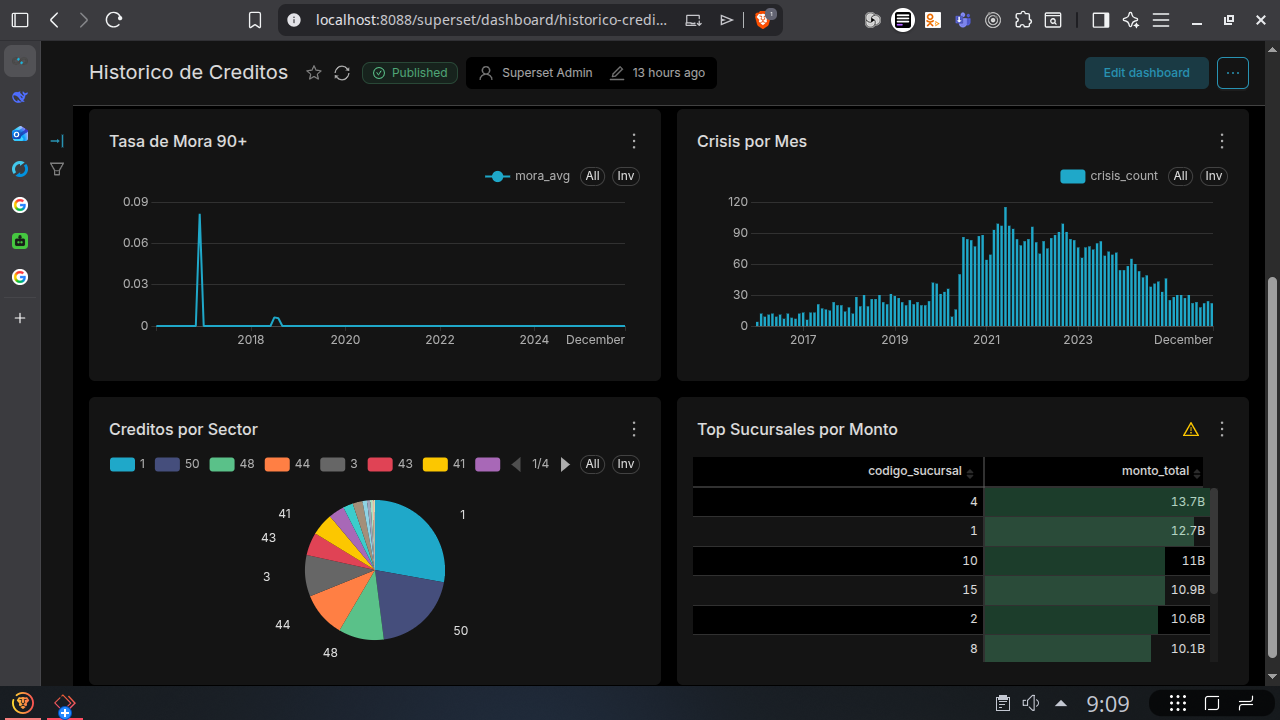
\includegraphics[width=0.8\textwidth]{images/dw-01-historicoCreditos2.png}
    \caption{Vista complementaria del dashboard histórico de créditos.}
    \label{fig:appendix_historico}
\end{figure}

\begin{figure}[h!]
    \centering
    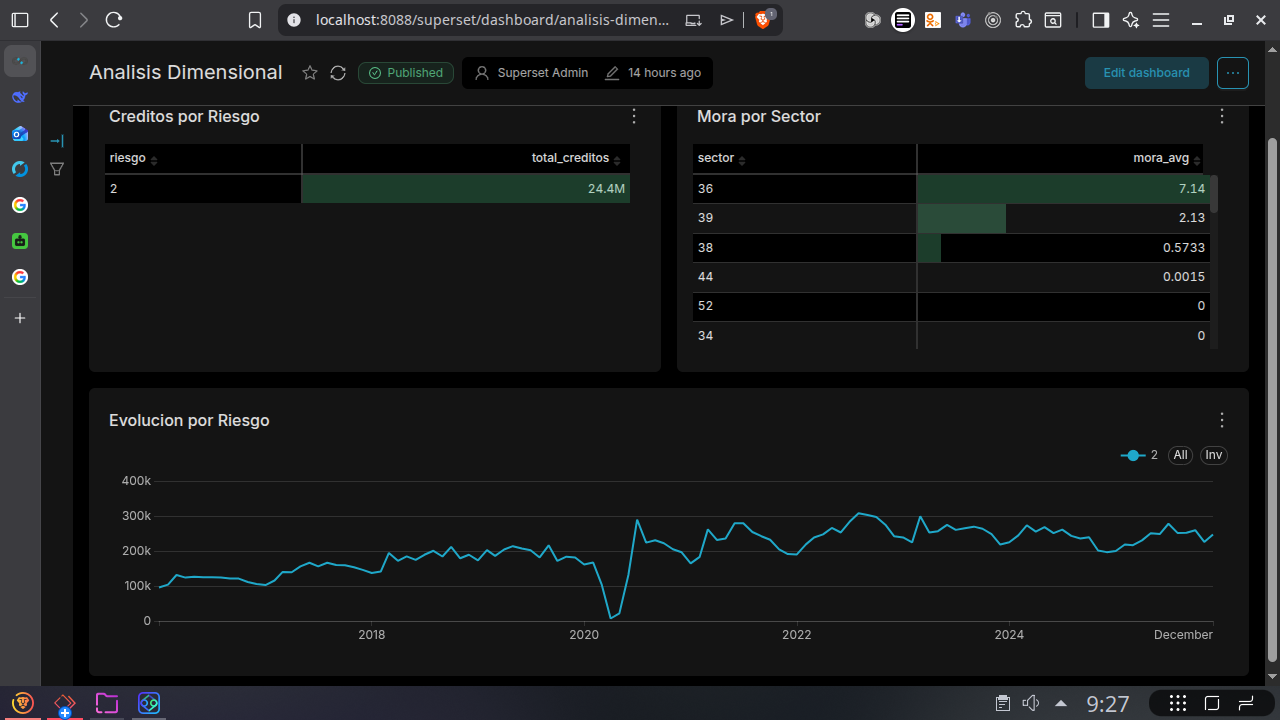
\includegraphics[width=0.8\textwidth]{images/dw-02-AnalisisDimensional.png}
    \caption{Dashboard de análisis dimensional por riesgo y sector.}
    \label{fig:appendix_dimensional}
\end{figure}

\begin{figure}[h!]
    \centering
    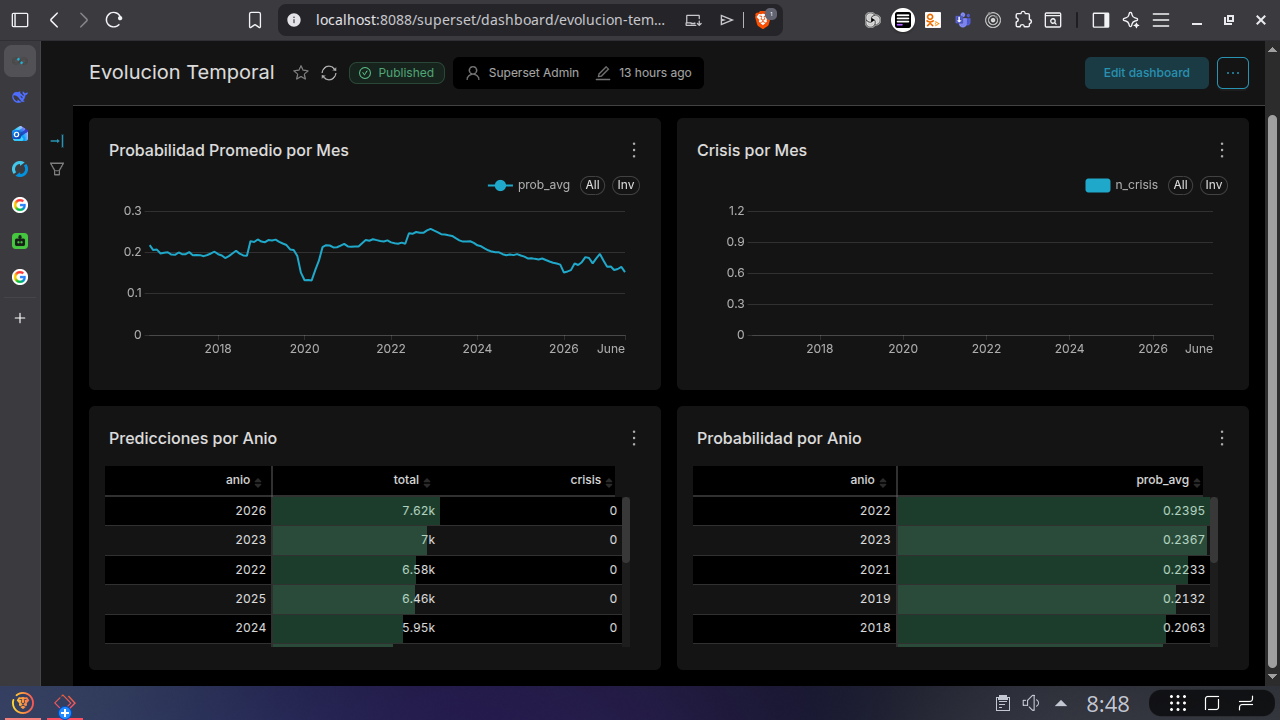
\includegraphics[width=0.8\textwidth]{images/dw-06-evolucionTemporal.png}
    \caption{Dashboard de evolución temporal de predicciones.}
    \label{fig:appendix_evolucion}
\end{figure}

\section{Información mínima para reproducibilidad}

La documentación final del repositorio debería incluir: definición de las ocho reglas de \texttt{crisis\_flag}; diccionario de las veintiuna características; conteos de registros y secuencias por etapa; particiones temporales; configuración completa de CNN, MLP y LightGBM; semillas; versiones de librerías; especificaciones de hardware; hashes o versiones de datos; métricas por horizonte; y procedimientos para ejecutar los DAG y reconstruir los dashboards.

\section{Esquema estrella del datamart}

El datamart analítico utiliza un esquema estrella con dos tablas de hechos que comparten las mismas dimensiones. A continuación se presentan los diagramas de cada tabla de hechos.

\subsection{Tabla de hechos: fact\_creditos\_mensual}

\begin{figure}[h!]
    \centering
    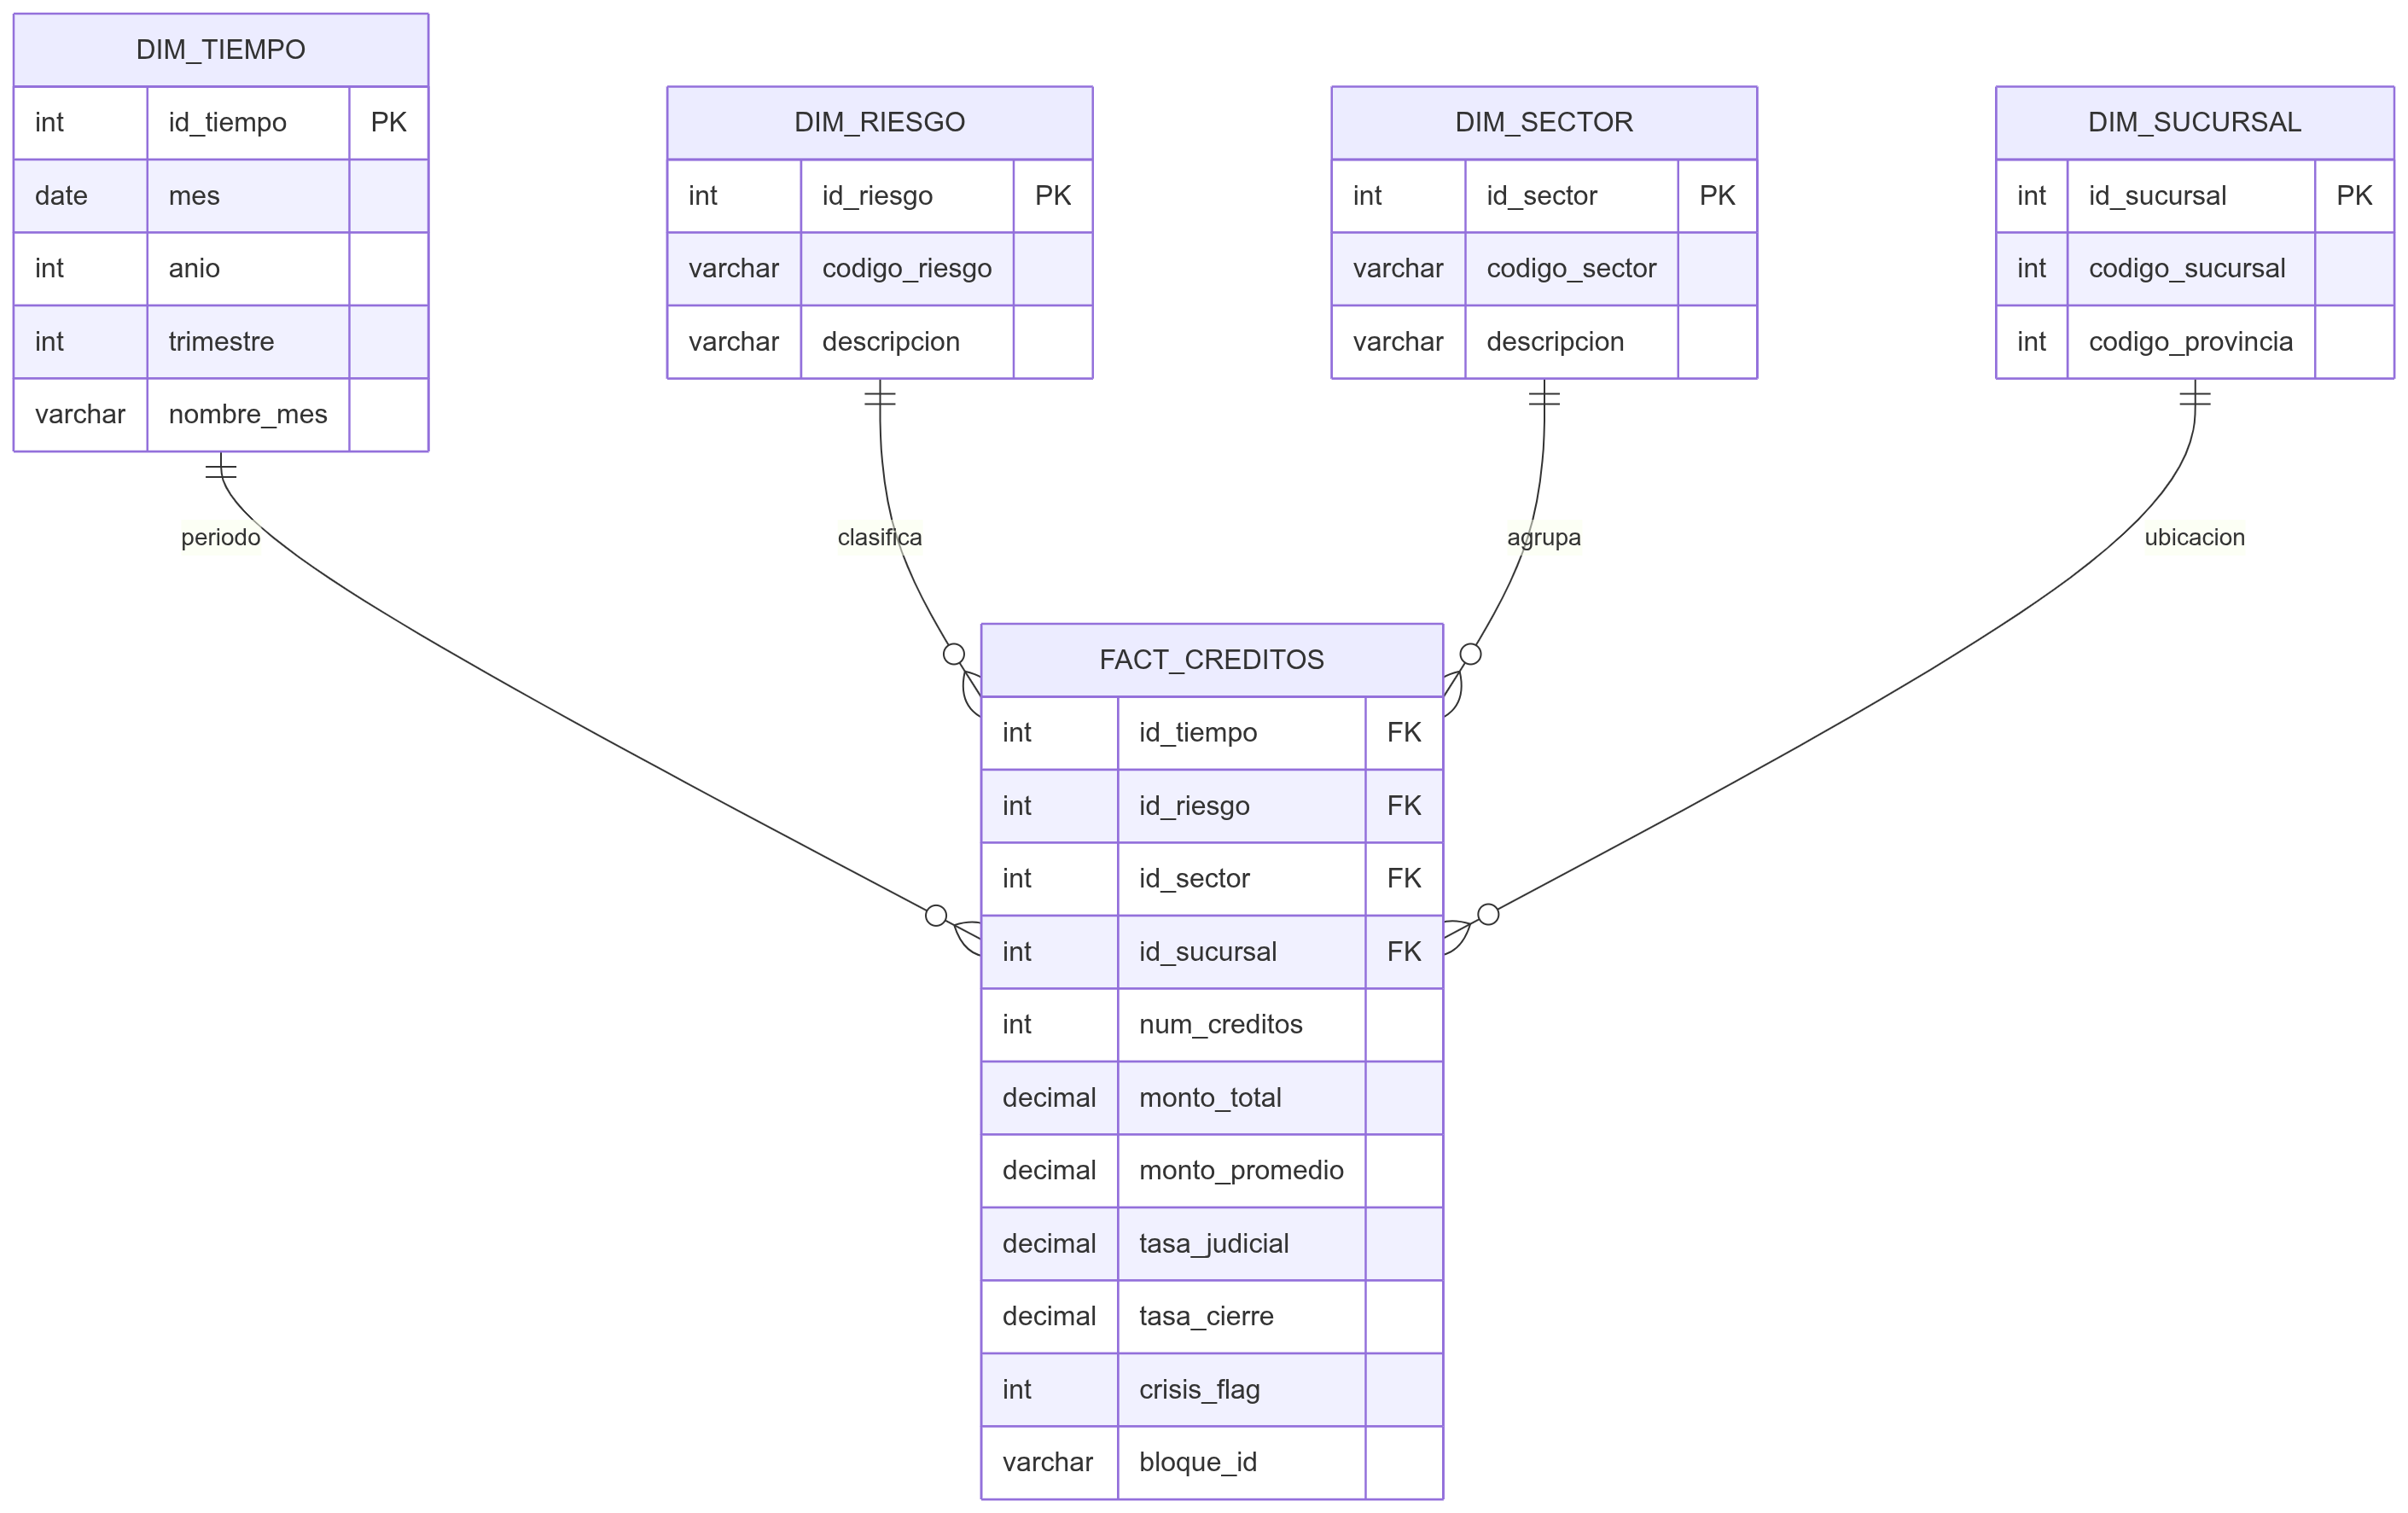
\includegraphics[width=1.0\textwidth]{images/MM-08a Estrella para fact_creditos_mensual.png}
    \caption{Esquema estrella de la tabla \texttt{fact\_creditos\_mensual}. Almacena los agregados históricos de créditos por bloque-mes, incluyendo la variable objetivo \texttt{crisis\_flag}.}
    \label{fig:appendix_estrella_creditos}
\end{figure}

\subsection{Tabla de hechos: fact\_predicciones}

\begin{figure}[h!]
    \centering
    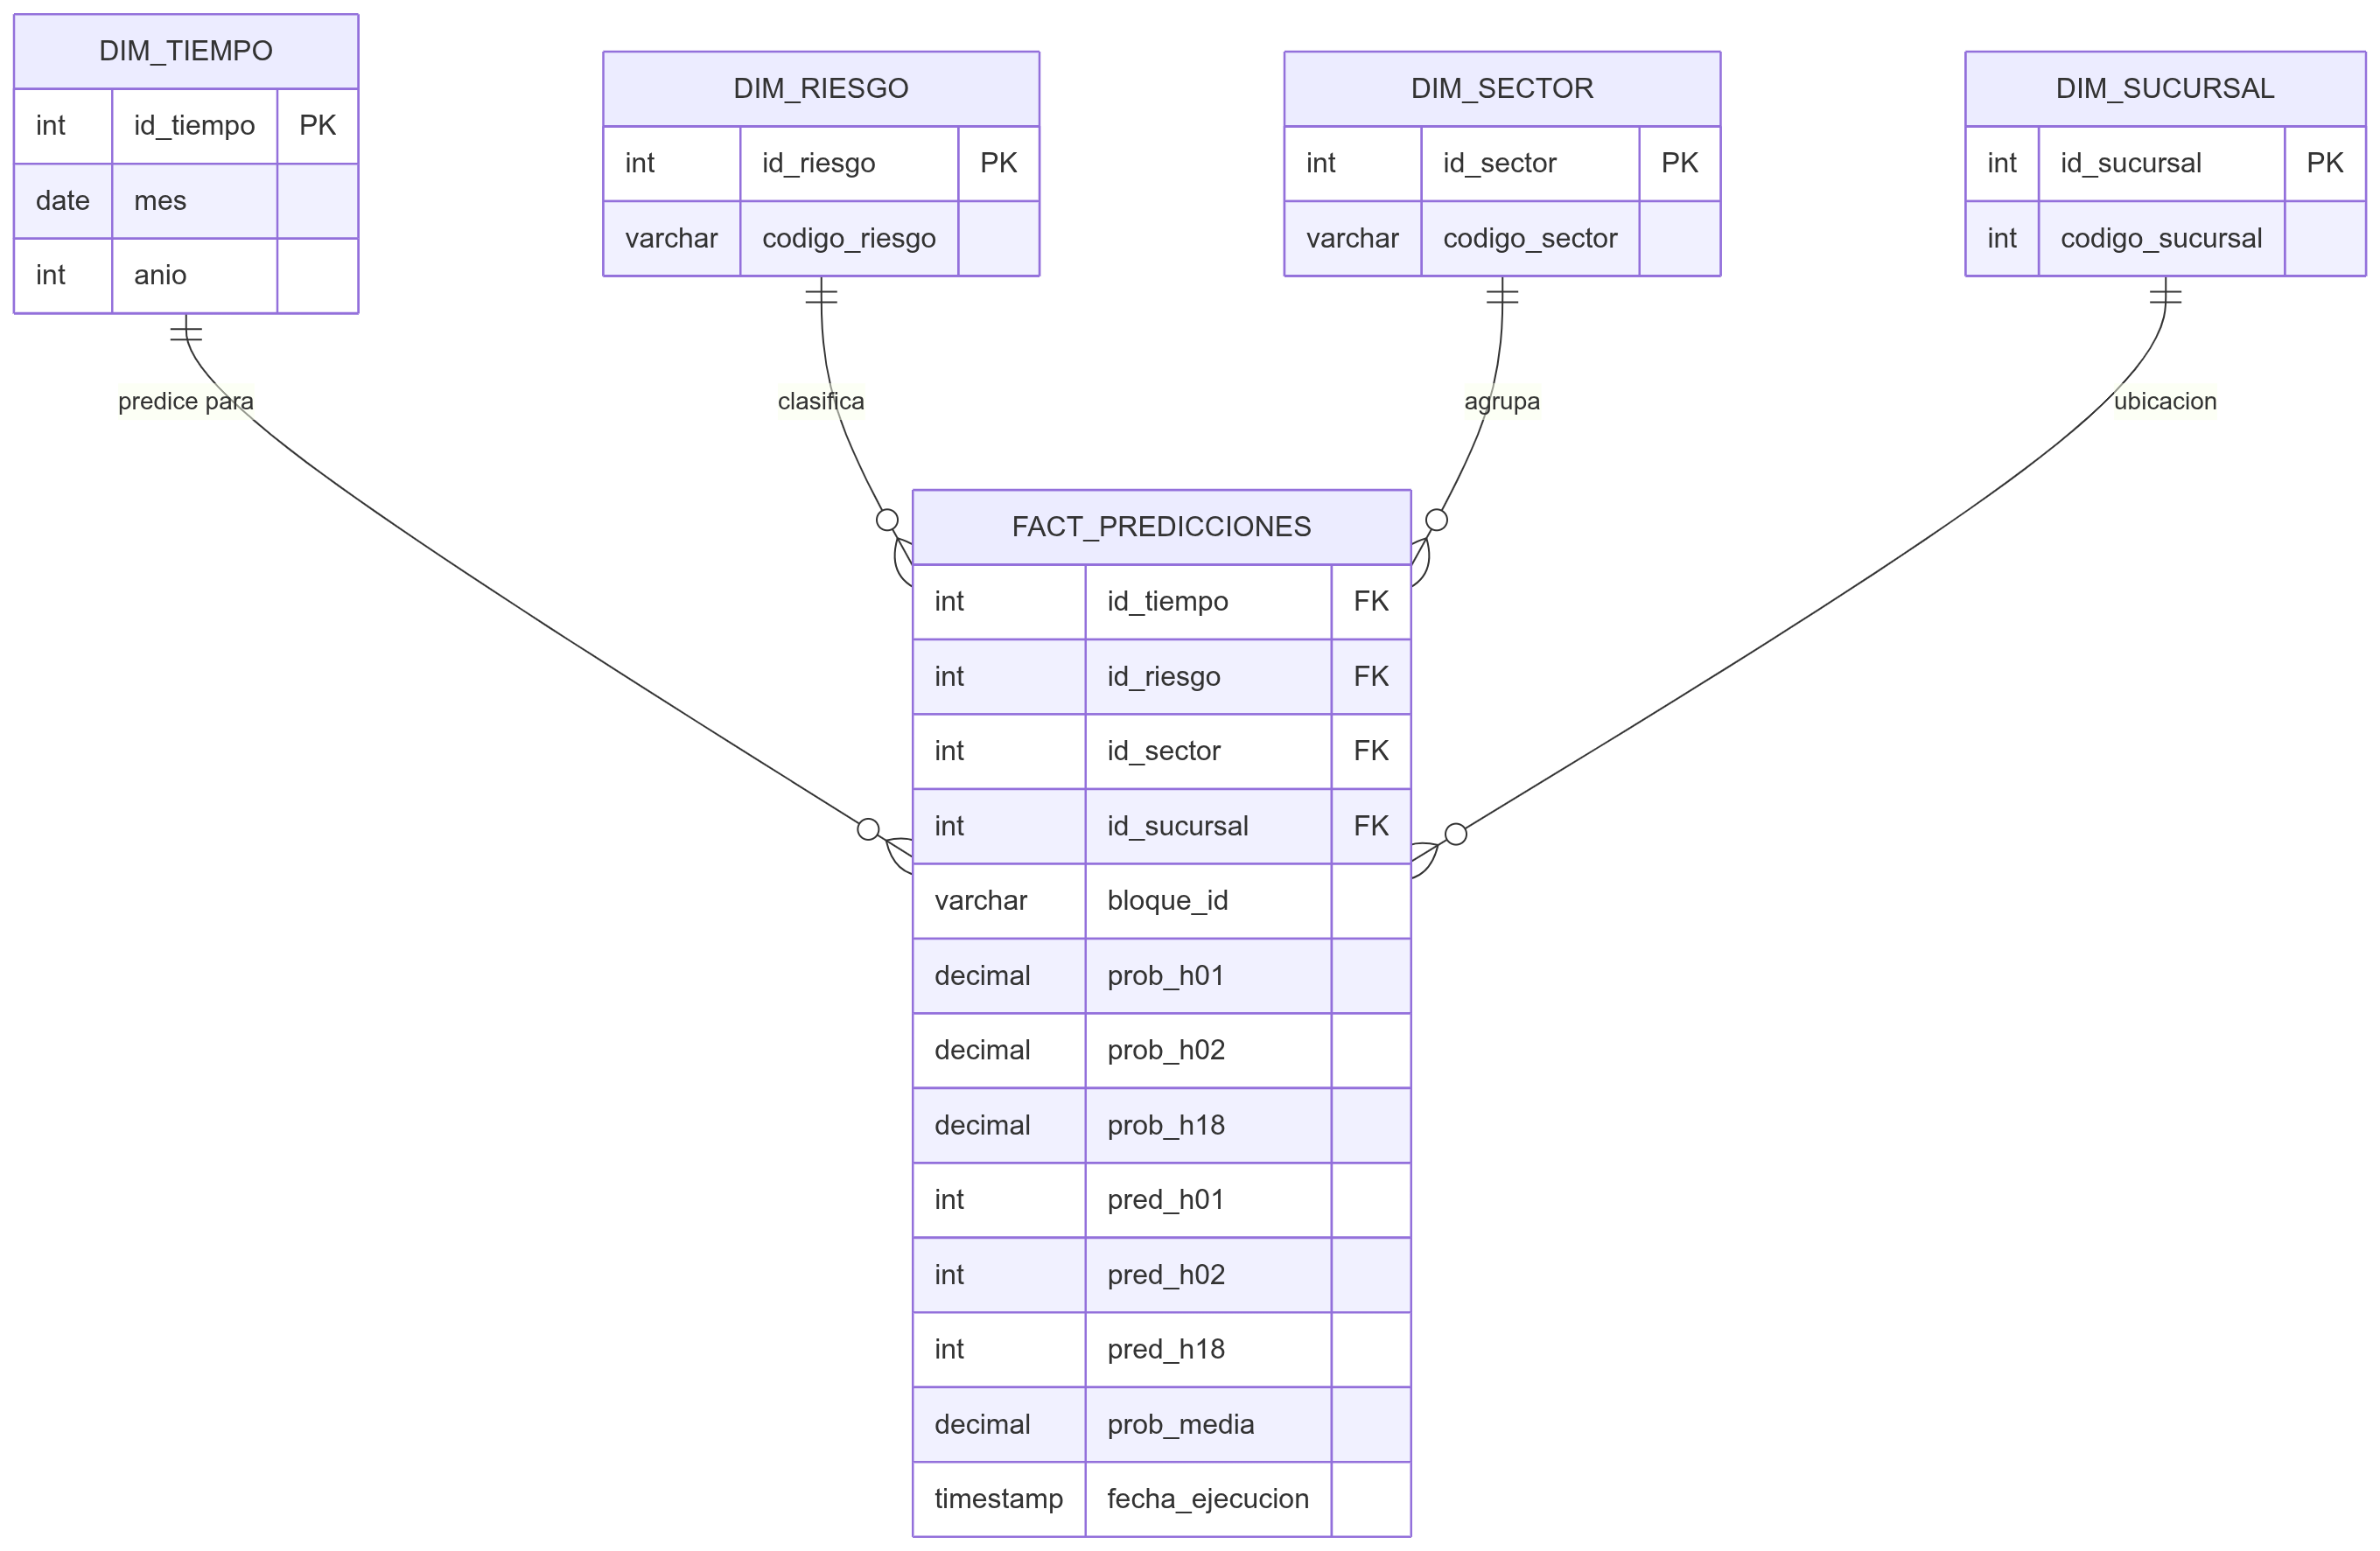
\includegraphics[width=1.0\textwidth]{images/MM-8b Estrella para fact_predicciones.png}
    \caption{Esquema estrella de la tabla \texttt{fact\_predicciones}. Almacena las probabilidades y predicciones binarias para los 18 horizontes temporales, generadas por el modelo seleccionado.}
    \label{fig:appendix_estrella_predicciones}
\end{figure}